\documentclass{controle}
\usepackage{main}

\title{Contrôle n°5 : Arithmétiques, décimaux, rationnels, variation et signe de fonctions}
\author{Seconde 3}
\date{17 Avril 2026}

\begin{document}
\titleandname{}
\instructions[autorisée]

\begin{questions}
\titledquestion{Variations et signes de fonctions}[5]
\begin{parts}
\part[3] Compléter les tableaux de variation des fonctions suivantes :
\vspace*{0.25cm}
\begin{subparts}
\begin{minipage}{0.4\textwidth}
\subpart[1] $f : x \mapsto 9x - 27$
\vspace*{0.1cm}
\begin{center}
\begin{tikzpicture}
\tkzTabInit{$x$ / 1, Variations de $f$ / 2}{$-\infty$, $+\infty$};
\end{tikzpicture}
\end{center}
\end{minipage}
\hfill
\begin{minipage}{0.4\textwidth}
\subpart[1] $g : x \mapsto -x + 8$
\vspace*{0.1cm}
\begin{center}
\begin{tikzpicture}
\tkzTabInit{$x$ / 1, Variations de $g$ / 2}{$-\infty$, $+\infty$};
\end{tikzpicture}
\end{center}
\end{minipage}
\vspace*{0.25cm}
\subpart $h$ est la fonction carrée définie sur $\R$.
\vspace*{0.1cm}
\begin{center}
\begin{tikzpicture}
\tkzTabInit{$x$ / 1, Variations de $h$ / 2}{$-\infty$, $+\infty$};
\end{tikzpicture}
\end{center}
\end{subparts}
\vspace*{0.25cm}
\part[2] Résoudre dans $\R$ les inéquations suivantes. On donnera l'ensemble $S$ des solutions de l'inéquation sous forme d'intervalle.
\begin{subparts}
\subpart $-8x + 56 \leq 0$
\subpart $x - 8 > 3x + 16$
\end{subparts}
\end{parts}

\newpage

\titledquestion{Nombres premiers}[4]
\begin{parts}
\part[2] Donner la décomposition en facteurs premiers des nombres suivants :
\begin{subparts}
\subpart $2088$
\subpart $\py{3*3*5*7*11}$
\subpart $\py{2*11*13}$
\subpart $\py{2*2*2*3*5*37}$
\end{subparts}

\vspace*{0.2cm}

\part[2] Soit $p$ un nombre premier. Démontrer que $p^2$ n'est pas un nombre premier.
\end{parts}

\vspace*{0.5cm}

\titledquestion{Multiples et diviseurs}[6]
\begin{parts}
\part[2] Donner la liste de tous les diviseurs positifs des nombres suivants :
\begin{subparts}
\subpart 147
\subpart 148
\subpart 164
\subpart 598
\end{subparts}

\vspace*{0.2cm}

\part On souhaite démontrer la proposition suivante :
\begin{tcolorbox}
La somme de trois entiers consécutifs est un multiple de $3$.
\end{tcolorbox}

\vspace*{0.2cm}

\begin{subparts}
\subpart[1] Tester la proposition avec les trois entiers consécutifs $25$; $26$ et $27$.
\subpart[0.5] Soit $n$ un entier. À quoi correspond l'expression $n + (n + 1) + (n + 2)$ dans le cadre de la proposition ?
\subpart[0.5] Simplifier cette expression. Peut-on la factoriser par $3$ ?
\subpart[1] Déduire de la réponse précédente que la proposition est vraie.
\subpart[1] La somme de \textit{quatre} entiers consécutifs est-elle forcément un multiple de $4$ ? Justifier votre réponse.
\end{subparts}
\end{parts}

\titledquestion{Rationnels et décimaux}[5]
\begin{parts}
\part[0.5] Donner l'exemple d'un nombre irrationnel (qui n'est pas rationnel).
\part[2] Pour chacune des fractions suivantes, déterminer lesquelles sont décimales. Justifier votre réponse.
\begin{subparts}
\subpart $\dfrac{21}{28}$
\subpart $\dfrac{38}{64}$
\subpart $\dfrac{18}{210}$
\subpart $\dfrac{39}{75}$
\end{subparts}

\vspace*{0.2cm}

\part[2.5] On s'intéresse au nombre $q = 0,9999\dots$, où le chiffre $9$ se répète à l'infini.
\begin{subparts}
\subpart Le nombre $q$ semble-t-il décimal ?
\subpart Montrer que $10q = q + 9$.
\subpart Résoudre l'équation $10x = x + 9$. En déduire une autre valeur de $q$. 
\end{subparts}
\end{parts}
\end{questions}
\end{document}